\documentclass{article}

\PassOptionsToPackage{numbers,compress}{natbib}
\usepackage[preprint]{neurips_2023}

\usepackage[utf8]{inputenc}
\usepackage[T1]{fontenc}
\usepackage{hyperref}
\usepackage{url}
\usepackage{booktabs}
\usepackage{amsfonts}
\usepackage{amsmath}
\usepackage{amsthm}
\usepackage{nicefrac}
\usepackage{microtype}
\usepackage{graphicx}
\usepackage{caption}
\usepackage{float}
\usepackage{xcolor}

\graphicspath{{../reports/figures/}}

\theoremstyle{plain}
\newtheorem{theorem}{Theorem}
\newtheorem{proposition}[theorem]{Proposition}
\newtheorem{corollary}[theorem]{Corollary}
\newtheorem{lemma}[theorem]{Lemma}
\theoremstyle{definition}
\newtheorem{remark}[theorem]{Remark}

\makeatletter
\renewcommand{\@noticestring}{%
  Preprint. Code, pinned data, and one script per reported number:
  \url{https://github.com/ITheClixs/crypto-return-predictability}%
}
\makeatother

\hypersetup{colorlinks=true, linkcolor=black, citecolor=black, urlcolor=blue!60!black}

\newcommand{\rsq}{R^2_{OS}}
\newcommand{\ir}{\mathrm{IR}}

\title{A Century Is Not Enough:\\Certification Bounds for Out-of-Sample Return Predictability}

\author{%
  Mehmet Demir Guven\thanks{%
    Independent work. The author is affiliated with ETH Z\"urich, but this research was
    carried out independently of it: it was not funded, supervised, commissioned or endorsed
    by ETH Z\"urich or by any other institution or firm, and no collaborator contributed to
    it.} \\
  Department of Computer Science \\
  ETH Z\"urich \\
  Universit\"atstrasse 6, 8092 Z\"urich, Switzerland \\
  \texttt{demirguven178@gmail.com} \\
}

\begin{document}

\maketitle

\begin{abstract}
  How precisely can a century-scale equity-premium dataset constrain economically meaningful
  out-of-sample predictability? We first state a minimum detectable effect under an explicit
  Gaussian constant-effect benchmark: for a one-sided test at size $\alpha$ and target power
  $\pi$, the smallest annualised information ratio detectable from $T$ years of \emph{evaluation}
  is $[z_{1-\alpha}+z_\pi]/\sqrt{T}$. This is a model-based power calculation, not a
  distribution-free impossibility bound. Because the design reserves twenty years for
  initialisation, the 1926--2025 data give at most eighty years of out-of-sample evaluation, so
  the detectable ratio is $0.28$ for one prespecified predictor and $0.44$ after Bonferroni
  correction over the forty-six candidates \citet{goyal2024} examine---against Campbell and
  Thompson's economic-significance threshold of $0.246$. The design is short by twenty-three
  years for a single test and by one hundred and seventy-three once the search is priced.
  We then apply a drift-robust, anytime-valid certificate to $117$ predictor--frequency pairs.
  Under the primary specification no pair reaches the individual $5\%$ threshold and none
  survives e-BH; across nine design specifications applied to the fourteen classic monthly
  predictors, none does either. Among the $116$ unflagged pairs the median of the \emph{marginal}
  $95\%$ upper endpoints is $0.60$ and $112$ exceed $0.25$, so most intervals remain compatible
  both with no incremental predictability and with effects conventionally called economically
  meaningful. Sequential paths show the accumulation is highly uneven across predictors and
  across time: of six classic predictors, only inflation accumulates evidence in both halves of
  the window, the Treasury-bill rate only in the second, the term spread gains in the first and
  surrenders it in the second, and the three valuation ratios accumulate in neither. These
  describe when the procedure gathered evidence and are not estimates of structural-break
  dates.
\end{abstract}

\section{Introduction}

The out-of-sample predictability literature asks whether a variable forecasts the equity
premium. After \citet{welch2008} the consensus answer is mostly no, and after
\citet{goyal2024} it is mostly no again for a further twenty-nine candidates. This paper asks
a prior question that determines what any such answer can mean: \emph{given a sample of a
certain length, what size of effect could it have detected at all?}

Under an explicit Gaussian constant-effect benchmark the question has a closed-form answer, and
it is uncomfortable. Section~\ref{sec:bound} derives a minimum detectable effect: the smallest
annualised information ratio a design evaluating $T$ years can detect at level $\alpha$ with
power $\pi$. It is a power calculation under a stated model, not a distribution-free
impossibility theorem, and Remark~\ref{rem:notimpossibility} says so precisely. Two features of
it matter. The floor scales with
$1/\sqrt{T}$ in \emph{calendar span} and is almost unaffected by sampling frequency, so a
century of monthly data and a century of annual data face nearly the same bound despite a
twelvefold difference in observations. And it degrades with the size of the search, which in
this literature is large and known.

Put those together against the effect the literature itself treats as meaningful---%
\citet{campbell2008} take a monthly out-of-sample $\rsq$ of $0.5\%$, an annualised information
ratio of $0.246$, as economically significant---and the arithmetic is stark. Under the
Gaussian benchmark of Section~\ref{sec:bound}, a single predictor needs $103$ years of
\emph{evaluation} to reach $80\%$ power against it, and $253$ once the $46$-predictor search
\citet{goyal2024} ran is priced. The canonical dataset begins in 1926 and the design reserves
its first twenty years, leaving eighty.

\paragraph{What we do with that.} A bound on what a study could have found is only useful if
paired with a bound on what it did find. Section~\ref{sec:instrument} uses an anytime-valid
\emph{certificate} \citep{guven2026}, a non-negative wealth process whose validity is a
finite-sample theorem and whose logarithm is the profit and loss of an explicit drift-hedged
strategy. Two properties earn its place here. It supplies a time-uniform \emph{ceiling} on a
predictor's incremental value, which is the number this literature has never reported and the
one a reader can act on. And because evidence compounds rather than averages, its path records
\emph{when} evidence arrived: a covariance averaged over a century weights an early
contribution and a late one identically, whereas a compounding process does not. We read the
path as a description of the procedure's evidence accumulation, not as an estimate of a
break date.

\paragraph{What we find.} Across $117$ predictor--frequency pairs from 1926 to 2025, nothing
is certified, under any of nine specifications of burn-in, window and payoff. That is
unsurprising and is not the contribution. The contribution is the interval: across the $116$
unflagged pairs the median of the \emph{marginal} $95\%$ upper endpoints on the incremental
annualised information ratio is $0.60$, and $112$ of them sit above Campbell and Thompson's
$0.25$. These are pairwise bounds, not a simultaneous statement about a median parameter. Read
as such they say that for almost every predictor in the set, the data rule out neither zero nor
an economically meaningful edge.

The timing result is secondary and needs stating carefully. Across all $117$ pairs, Clark--West
statistics and certificate e-values are \emph{positively} rank correlated, at a Spearman
coefficient of $+0.54$ ($+0.55$ over the $116$ unflagged). The two are measuring overlapping
things, as they should. Among six classic predictors we display for illustration they disagree
sharply, at $-0.83$; that subset shows the two \emph{can} diverge and why, not that they
generally invert. Read on the certificate's underlying process, the three valuation ratios---the
predictors Clark--West scores highest, at $1.34$ to $1.64$---accumulate no evidence in either
half of the window, while inflation, the Treasury-bill rate and the term spread do, in different
halves. A statistic that averages a covariance over a century weights the two halves equally; a
process that compounds does not, and the difference is visible.

\paragraph{What this is not.} We do not claim the certificate is more powerful than
Clark--West. It is not: \citet{guven2026} measures the exchange rate at roughly a factor of two
in sample size, the price of validity at every stopping time and under weaker assumptions. Nor
do we claim to overturn \citet{welch2008}; we agree with it and reproduce it. The claim is
narrower and, we think, more useful: this literature has been operating at or below the
detection threshold of its own data for its entire history, the threshold is computable in
advance, and the quantity worth reporting is a ceiling rather than a $p$-value.

\section{Related work}
\label{sec:related}

\paragraph{The predictability literature and its instability.} \citet{welch2008} evaluate
seventeen predictors of the equity premium and find that essentially none beats the historical
mean out of sample; \citet{goyal2024} repeat the exercise for twenty-nine further candidates
published since, and reach the same verdict for most of them. \citet{campbell2008} argue that
weak predictability can still be economically meaningful once forecasts are constrained by
economic priors, and set the benchmark effect size we use throughout.
\citet{rapach2010} recover out-of-sample gains from forecast combination. Running underneath
all of it is instability: the same predictor works in one era and not the next, which is the
observation the sequential paths of Section~\ref{sec:results} illustrate and
Proposition~\ref{prop:intermittent} prices.

\paragraph{Power, and what a test can be expected to find.} \citet{inoue2005} show that
out-of-sample tests are typically \emph{less} powerful than in-sample ones, because splitting
a finite sample costs information, and warn against reading out-of-sample failure as evidence
that in-sample evidence was spurious. Our contribution is complementary and more absolute:
their comparison is between two procedures on the same data, whereas
Proposition~\ref{prop:floor} asks what a span of a given length can support at a stated size and
power under a stated model---a design question rather than a procedure comparison. It is not a
statement about all procedures, and Remark~\ref{rem:notimpossibility} draws that line. \citet{hansen2011} address a related selection problem by constructing a set of
models that cannot be distinguished from the best. Where a model confidence set answers ``which of
these can be told apart'', we ask ``could any of them have been told apart from nothing, given
this much data''. We also run their procedure on our own forecasts in
Section~\ref{sec:toolkit}, where it retains every model including the benchmark.

\paragraph{Nested forecast comparison.} \citet{diebold1995} is not valid for nested models;
\citet{clark2001} and \citet{clark2006, clark2007} supply the corrections this literature uses,
and \citet{guven2026} shows that the benchmark against which the correction is applied
determines what null is being tested. We use Clark--West throughout as the incumbent and do
not propose to replace it.

\paragraph{Game-theoretic statistics.} The certificate is built from test martingales and
e-values \citep{ville1939, shafer2019, ramdas2023, waudbysmith2024}, with merging rules from
\citet{vovk2021} and false-discovery control from \citet{wang2022}. Applications of betting
arguments to finance exist---\citet{kumon2011} test whether observed \emph{price processes} are
martingales using limit-order betting strategies---but that is a specification test of the
price process rather than a comparison of a forecasting model against an estimated benchmark,
and it does not treat the drift as a nuisance. We are not aware of prior anytime-valid analysis
of equity-premium predictability.

\section{The certification bound}
\label{sec:bound}

Let a signal-weighted strategy have annualised information ratio $\ir$, and consider testing
whether $\ir > 0$ from $T$ years of data at level $\alpha$.

\begin{proposition}[Gaussian minimum detectable information ratio]
\label{prop:floor}
Let $X_1,\dots,X_n$ be independent Gaussian strategy returns with mean $\mu$ and known variance
$\sigma^2$, let there be $P$ observations per year, let $n=PT$, and define the annualised
information ratio $\rho=\sqrt{P}\,\mu/\sigma$. For the one-sided test of $H_0:\mu\le0$ against
$H_1:\mu>0$ at size $\alpha$, the uniformly most powerful test rejects when
$\sqrt{n}\,\bar X/\sigma \ge z_{1-\alpha}$, and its power is
\[
  \pi(\rho,T) \;=\; \Phi\!\big(\rho\sqrt{T}-z_{1-\alpha}\big).
\]
The smallest annualised ratio attaining target power $\pi$ from $T$ years of evaluation is
therefore
\[
  \rho_{\mathrm{MDE}}(T,\alpha,\pi) \;=\; \frac{z_{1-\alpha}+z_\pi}{\sqrt{T}},
\]
and the span needed against a given $\rho$ is $[z_{1-\alpha}+z_\pi]^2/\rho^2$. For $m$
prespecified hypotheses under Bonferroni, replace $\alpha$ by $\alpha/m$.
\end{proposition}

We write \emph{floor} for $\rho_{\mathrm{MDE}}$ throughout, as shorthand for ``the minimum
detectable ratio of this design at this size and power''. It is a property of a design, not of
the class of all procedures; Remark~\ref{rem:notimpossibility} states the difference and we do
not use the word in the stronger sense anywhere.

\begin{remark}[What this is and is not]
\label{rem:notimpossibility}
Proposition~\ref{prop:floor} is a design-stage power calculation under a stated model, not a
distribution-free lower bound over all procedures. Effects below $\rho_{\mathrm{MDE}}$ can still
produce rejection; they do so with probability below $\pi$. The calculation assumes independent
Gaussian returns, a constant effect, known variance, and a strategy fixed in advance; with
serial dependence $\sigma^2$ must be replaced by a long-run variance, and with an estimated
variance the finite-sample distribution is noncentral $t$ rather than normal. A genuinely
procedure-independent statement would require a minimax or information-theoretic argument under
a specified experiment, which we do not attempt. We use the benchmark because it is the
calculation the applied literature would itself perform, not because it is the sharpest
available.
\end{remark}

\begin{corollary}[Frequency invariance under square-root-of-time scaling]
\label{cor:frequency}
Under the assumptions of Proposition~\ref{prop:floor}---independent increments, a constant
effect, non-overlapping observations, and mean and variance scaling as $P$ and $\sqrt{P}$ so
that $\rho$ is preserved---$\rho_{\mathrm{MDE}}$ depends on the calendar span $T$ and not on the
number $P$ of observations per year.
\end{corollary}

The cancellation is exact only under those assumptions. It need not hold under serial
correlation, overlapping observations, conditional heteroskedasticity, recursive estimation,
predictor persistence, or when lower-frequency series carry information that higher-frequency
ones do not. Section~\ref{sec:results} reports that the measured thresholds are numerically
close across frequencies in this dataset, which is evidence that the approximation is adequate
here and not a proof that it holds generally.

Proposition~\ref{prop:floor} assumes the effect is present throughout. It is not, in this
literature, and the correction is unfavourable.

\begin{proposition}[Intermittent effects raise the detectable threshold]
\label{prop:intermittent}
Let $I_t\in\{0,1\}$ be an indicator, independent of the innovation, with $P(I_t=1)=\phi$, and
let $y_t=m I_t+\varepsilon_t$ with $\mathbb{E}[\varepsilon_t]=0$ and
$\operatorname{Var}(\varepsilon_t)=\sigma^2$. For a strategy sized on $g_t=mI_t$, the
per-period payoff $X_t=g_ty_t$ has $\mathbb{E}[X_t]=\phi m^2$ and
$\operatorname{Var}(X_t)=\phi m^2\sigma^2+\phi(1-\phi)m^4$, so with
$\rho_{\mathrm{on}}=m/\sigma$ the per-period ratio is
\[
  \rho_{\mathrm{measured}}
  \;=\; \frac{\sqrt{\phi}\,\rho_{\mathrm{on}}}
             {\sqrt{1+(1-\phi)\rho_{\mathrm{on}}^{2}}}
  \;\approx\; \sqrt{\phi}\,\rho_{\mathrm{on}}
  \qquad\text{for small }\rho_{\mathrm{on}},
\]
and under that approximation the span required scales as $1/(\phi\,\rho_{\mathrm{on}}^2)$: a
factor $1/\phi$ longer than for an always-present effect of the same on-period strength.
\end{proposition}

The second denominator term is the variance contributed by switching between regimes, and it is
not negligible in general: at a per-period $\rho_{\mathrm{on}}$ of $0.58$ the approximation
overstates the ratio by up to $14\%$ across duty cycles, and at $1.7$ by up to $90\%$, in both
cases worst at the smallest $\phi$. At the magnitudes this paper uses it is negligible---an
annualised on-period ratio of $0.5$ is a per-period $0.14$ at monthly frequency, where the
error stays under $1\%$ for every $\phi$. We confirm the exact expression against four million
simulated periods at each of seven duty cycles and three ratios; the largest discrepancy is
$0.99\%$ and occurs where Monte Carlo noise dominates. The strategy also has to be able
to size on $I_t$, which requires the regime to be known in advance; where it is not, the
achievable ratio is lower still, so the approximation errs in the direction that understates
the problem.

\begin{remark}[We do not estimate $\phi$ from the wealth path]
\label{rem:nophi}
It is tempting to read a duty cycle off the interval between the start of evaluation and the
year the certificate's wealth peaks, and an earlier draft did. We do not. The peak is a random,
post-hoc quantity that depends on noise, stake calibration and the payoff; it is not a
changepoint estimator and carries no interval. Where a duty cycle appears below it is measured
as the fraction of equal sub-periods with positive accumulation---a descriptive statistic---or
supplied externally as a hypothetical.
\end{remark}

\begin{table}[t]
  \centering
  \caption{Minimum detectable annualised information ratio at $80\%$ power, and the evaluation
  span needed against Campbell and Thompson's economic-significance threshold. Every entry comes
  from one script (\texttt{goyal\_welch\_mde.py}) and the same expressions. The threshold is
  reported unrounded at $0.2456$: rounding it to $0.25$ shortens the required span by about four
  years. The data span 100 calendar years, but the twenty-year initialisation leaves at most
  \textbf{80} years of out-of-sample evaluation, which is the span the test actually has.}
  \label{tab:floor}
  \small
  \begin{tabular}{lrrrr}
    \toprule
    Correction & $\alpha$ & MDE at 80 y & MDE at 100 y & Years needed for $\rho=0.2456$ \\
    \midrule
    One predictor                  & $0.0500$ & $0.278$ & $0.249$ & $103$ \\
    Bonferroni over 17 \citep{welch2008} & $0.0029$ & $0.402$ & $0.360$ & $214$ \\
    Bonferroni over 46 \citep{goyal2024} & $0.0011$ & $0.437$ & $0.391$ & $253$ \\
    Bonferroni over 100            & $0.0005$ & $0.462$ & $0.413$ & $283$ \\
    \midrule
    \multicolumn{5}{l}{\emph{Available evaluation span: 80 years. Short by 23 years for one
    test, 173 corrected.}} \\
    \bottomrule
  \end{tabular}
\end{table}

Table~\ref{tab:floor} states the position, and the distinction between the raw and the
evaluation span matters. Against the raw hundred years a single test would sit within three
years of the boundary; against the eighty years the design actually evaluates it is short by
twenty-three, with no margin for parameter instability, transaction costs, or a slightly
smaller true effect. Corrected for the search that was performed, the shortfall is one hundred
and seventy-three years.


\paragraph{Reading the floor in the units the literature uses.} Table~\ref{tab:translation}
converts a monthly out-of-sample $\rsq$---the quantity this literature reports---into the
annualised information ratio the bound is stated in, and then into required span. The row that
matters is the third: Campbell and Thompson's threshold for economic significance corresponds
to an annualised ratio of $0.25$ and needs $103$ years for a single predictor, $253$ once the
search is corrected for. Even a monthly $\rsq$ of $1\%$, twice what that literature treats as
meaningful and larger than anything in our results, needs $126$ years under the correction.

\begin{table}[t]
  \centering
  \caption{The same effect in four currencies. Monthly out-of-sample $\rsq$ as reported by the
  literature; the implied per-period and annualised information ratios; and the calendar span a
  one-sided fixed-sample test needs to reach $80\%$ power against it, uncorrected and
  Bonferroni-corrected for the $46$-predictor search of \citet{goyal2024}.}
  \label{tab:translation}
  \small
  \begin{tabular}{rrrrr}
    \toprule
    Monthly $\rsq$ & Per-period $\ir$ & Annualised $\ir$ & Years, one test & Years, 46 tests \\
    \midrule
    $0.1\%$ & $0.032$ & $0.11$ & $515$ & $1271$ \\
    $0.2\%$ & $0.045$ & $0.16$ & $257$ & $635$ \\
    $0.5\%$ & $0.071$ & $0.25$ & $103$ & $253$ \\
    $1.0\%$ & $0.101$ & $0.35$ & $51$ & $126$ \\
    $2.0\%$ & $0.143$ & $0.49$ & $25$ & $62$ \\
    \bottomrule
\end{tabular}

\end{table}

\begin{figure}[t]
  \centering
  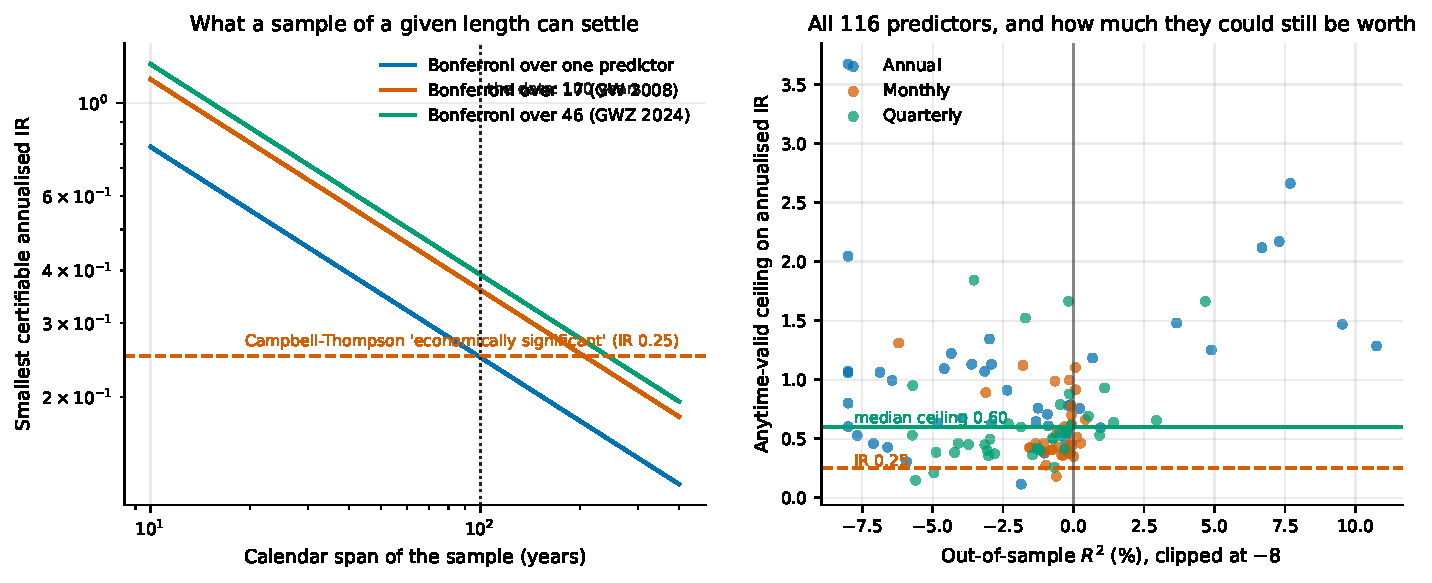
\includegraphics[width=\linewidth]{fig12_equity.pdf}
  \caption{\textbf{Left:} the minimum detectable ratio against evaluation span, for searches of one,
  seventeen and forty-six predictors. The horizontal line is Campbell and Thompson's
  economic-significance threshold; the vertical line is the data. \textbf{Right:} every
  predictor--frequency pair, plotted as its anytime-valid ceiling against its out-of-sample
  $\rsq$. The median of the marginal upper endpoints is $0.60$ and $112$ of $116$ lie above
  $0.25$: for almost every predictor the data rule out neither zero nor an economically
  meaningful edge.}
  \label{fig:equity}
\end{figure}

\section{The instrument}
\label{sec:instrument}

We use the drift-robust certificate of \citet{guven2026}. Because every number in
Section~\ref{sec:results} depends on it, we state the construction in full rather than by
reference.

\paragraph{Setup.} Let $\mathcal{F}_t$ be the filtration generated by everything observable
through the close of period $t$. The outcome $y_{t}$ is the period-$t$ log equity premium; the
signal $g_{t}$ is the period-$t$ forecast from the predictive regression minus the
intercept-only forecast from the \emph{same} estimation window, so $g_t$ is
$\mathcal{F}_{t-1}$-measurable and equals zero exactly when the two forecasts agree. Write
$\hat\sigma_{t}$ for the running standard deviation of the outcome through $t-1$ and
$z_t=g_t/\hat\sigma^{g}_{t}$ for the signal standardised by its own running scale, again using
only $\mathcal{F}_{t-1}$. The null is
\[
  H_0:\quad \mathbb{E}\!\left[\,y_t-\mu \,\middle|\, \mathcal{F}_{t-1}\right]=0
  \quad\text{for some fixed but unknown } \mu\in\mathbb{R},
\]
that is, the outcome is a martingale difference around \emph{some} drift and the signal carries
no information about it. The drift $\mu$ is a nuisance and is not assumed known.

\paragraph{Two martingales.} Fix a candidate drift $\mu$ and a payoff $\varphi$; throughout we
take $\varphi(u)=u$, the identity, which requires an a-priori envelope $B$ with $|y_t|\le B$ and
nothing else. Put $\psi_t(\mu)=\varphi\!\left((y_t-\mu)/\hat\sigma_t\right)$ and let
$E_t=\sup_u|\varphi(u)|$ over the reachable range be the corresponding payoff envelope. Define
\begin{align*}
  W^{\mathrm{sig}}_t(\mu) &= \prod_{s\le t}\bigl(1+\lambda_s\,g_s\,\psi_s(\mu)\bigr),
  &\lambda_s &\in \Bigl[0,\ \tfrac{c}{|g_s|E}\Bigr] \ \text{predictable},\\
  W^{\mathrm{ctr}}_t(\mu) &= \tfrac12\prod_{s\le t}\bigl(1+\kappa\psi_s(\mu)\bigr)
                        + \tfrac12\prod_{s\le t}\bigl(1-\kappa\psi_s(\mu)\bigr),
  &\kappa &= \tfrac{c'}{E},
\end{align*}
with $c=0.9$ and $c'=0.9$ so that every factor stays strictly positive. The first is the wealth
of a bettor who stakes a predictable fraction on the signal leading the outcome; the second is
the average of two bettors staking in opposite directions on $\mu$ being the wrong centre. The
stakes $\lambda_s$ are chosen by the usual predictable-mixture rule from the realised payoffs
through $s-1$, capped at $c/(|g_s|E)$; because they are $\mathcal{F}_{s-1}$-measurable, no
choice of $\lambda$ can affect validity, only power.

\paragraph{The certificate.} With $w=0.9$,
\[
  \mathcal{E}^{\,\mathrm{raw}}_t \;=\; \inf_{\mu\in\mathbb{R}}\;
  \Bigl[\,w\,W^{\mathrm{sig}}_t(\mu) + (1-w)\,W^{\mathrm{ctr}}_t(\mu)\,\Bigr],
  \qquad
  \mathcal{E}_t \;=\; \max_{s\le t}\ \mathcal{E}^{\,\mathrm{raw}}_s .
\]
Under $H_0$ each of $W^{\mathrm{sig}}_t(\mu^\star)$ and $W^{\mathrm{ctr}}_t(\mu^\star)$ is a
non-negative martingale at the true drift $\mu^\star$, hence so is their convex combination, and
an infimum over $\mu$ is bounded above by the value at $\mu^\star$. Ville's inequality gives
$P\bigl(\exists t:\mathcal{E}_t\ge1/\alpha\bigr)\le\alpha$ in finite samples, uniformly in time
and uniformly in the unknown drift. At a wrong $\mu$ the centring bettor gets rich, so the
infimum is not dragged to zero by candidates the data have already ruled out; the nuisance is
\emph{eliminated} rather than estimated, which is what removes the bootstrap.

Two numerical points matter and we state them because getting either wrong is silent. The
infimum is computed on a grid, and the grid spacing must resolve the drift to better than its
sampling error $\hat\sigma/\sqrt{n}$---a grid spaced at $\hat\sigma$ produces an infimum above
the true one and leaks type-I error. And $\mathcal{E}_t$ is the running maximum, which is the
object Ville's inequality bounds and the only one a test may use; $\mathcal{E}^{\,\mathrm{raw}}$
is the process itself and is the object any \emph{diagnostic} must use, since a running maximum
rises only when a new high is set. Table~\ref{tab:dating}, Figure~\ref{fig:dating} and
Section~\ref{sec:duty} all use $\mathcal{E}^{\,\mathrm{raw}}$.

\paragraph{From a certificate to a ceiling.} Inverting the same construction over a value
parameter, rather than testing it against zero, gives a time-uniform confidence interval for
\[
  \theta \;=\; \mathbb{E}\bigl[z_t\,(y_t-\mu)\bigr],
\]
the expected per-period return of a position sized by the standardised signal. For each
candidate $(\theta,\mu)$ a two-sided betting martingale tests $\mathbb{E}[z_t(y_t-\mu)]=\theta$;
it is averaged with the centring martingale as above, and $\theta$ is retained when the infimum
over $\mu$ never reaches $1/\alpha$. The retained set is an interval and its endpoints are found
by bisection. The following converts its upper endpoint into the units this literature uses.

\begin{lemma}[Value to annualised information ratio]
\label{lem:convert}
Let $\sigma_y$ be the outcome's standard deviation and $P$ the number of periods in a year.
A position taking $z_t$ units of the outcome earns $\theta$ per period in expectation with
per-period standard deviation $\sigma_y\sqrt{\mathbb{E}[z_t^2]}$, so its per-period information
ratio is $\theta/(\sigma_y\sqrt{\mathbb{E}[z_t^2]})$. The standardisation makes
$\mathbb{E}[z_t^2]\to1$, and under serially uncorrelated payoffs the ratio scales with the
square root of the aggregation, giving
\[
  \rho \;=\; \frac{\sqrt{P}\,\theta}{\sigma_y}.
\]
Applying this to the interval's upper endpoint gives the reported ceiling.
\end{lemma}

\begin{lemma}[Out-of-sample $\rsq$ to information ratio]
\label{lem:r2}
Let the benchmark forecast have mean-squared error $\sigma_y^2$ and let the model's incremental
forecast be $g_t$ with $\mathbb{E}[g_t^2]=\sigma_g^2$. Then
$\rsq = 1 - \mathbb{E}[(y_t-\hat y_t)^2]/\mathbb{E}[(y_t-\bar y)^2] = \sigma_g^2/\sigma_y^2$
when the incremental forecast is orthogonal to the benchmark error, and a position sized
proportionally to $g_t$ has per-period ratio $\sigma_g/\sigma_y=\sqrt{\rsq}$. Annualising,
\[
  \rho \;=\; \sqrt{P\,\rsq}.
\]
At $P=12$ and $\rsq=0.5\%$ this is $\rho=0.2450$; the $0.2456$ used in Table~\ref{tab:floor}
comes from the same calculation applied to the log-premium series' own moments.
\end{lemma}

Both conversions assume serially uncorrelated payoffs and unit-scale standardisation; neither is
exact and both are stated so a reader can check them against their own convention. They are the
only place a squared-error number and a betting number are made comparable, and every such
comparison in this paper routes through them.

\emph{Multiplicity without a bootstrap.} E-values average to an e-value under arbitrary
dependence, so the grid-level statistic over the $117$ dependent tests is their mean, and
false-discovery control follows from e-BH \citep{wang2022} with no assumption on the dependence
structure and no resampling.

\section{Data and design}
\label{sec:data}

We use the \citet{goyal2024} dataset through December 2025: monthly, quarterly and annual
equity-premium series from 1926 together with the seventeen classic \citet{welch2008}
predictors and the twenty-nine added by \citeauthor{goyal2024}. The outcome is the log equity
premium $\log(1+r_t)-\log(1+r^f_t)$; predictors are lagged one period; forecasts come from an
expanding-window OLS regression with an intercept, re-estimated every period, and the
benchmark is the same window's historical mean, which is that regression's intercept-only
restriction. Following \citeauthor{goyal2024}, the out-of-sample period begins twenty years
after the in-sample period starts.

\paragraph{Real-time versus revised series.} Many of the new predictors require re-estimation
every period, and \citeauthor{goyal2024} ship them as vintage matrices whose rows index the
period and whose columns index the vintage. The admissible series is the diagonal---what a
forecaster actually had---and the revised series is the last column. We use the diagonal
throughout and record the source per predictor. On the twenty-five predictors where both
exist, the revised series looks \emph{better} for only four, so this choice does not drive the
results; it is nonetheless the difference between an out-of-sample claim and a claim that
quietly uses full-sample parameter estimates.

\paragraph{Validation.} Because everything here depends on the pipeline being right, we
validate it against \citeauthor{goyal2024}'s published Table 3 Panel A, predictor by
predictor, matching their evaluation window and their Campbell--Thompson restriction. Across
the fourteen classic monthly predictors the correlation is $0.968$ (Spearman $0.959$), signs
agree in $13$ of $14$, and the median absolute gap is $0.075$ percentage points. The single
disagreement is $tms$, where both values round to zero.

\begin{remark}[The Campbell--Thompson restriction is not free]
Truncating the forecast at a non-negative equity premium helps $13$ of the $14$ predictors and
moves the mean out-of-sample $\rsq$ from $-0.511\%$ to $-0.281\%$. Since the effects under
discussion are themselves a few tenths of a percentage point, an economically motivated
truncation is doing about as much work as any predictor in the set. It helps most exactly
where the unrestricted regression produces the wildest forecast. We report unrestricted
numbers by default.
\end{remark}

\section{Results}
\label{sec:results}

\paragraph{Two grids, kept separate.} The \emph{primary} grid is the $117$
predictor--frequency pairs of Table~\ref{tab:full}, run once under the pre-specified design of
Section~\ref{sec:data}. The \emph{sensitivity} grid is a smaller object: the fourteen classic
monthly predictors, re-run under nine designs. The two are reported separately throughout,
because a maximum over $117$ pairs and a maximum over $14$ are not comparable quantities and an
earlier draft quoted one for the other.

\paragraph{Nothing is certified, and not for want of trying.} On the primary grid, out-of-sample
$\rsq$ is negative for $95$ of $117$ ($81\%$), no pair reaches the $\alpha=0.05$ threshold, the
largest e-value observed is $7.47$, the grid-level merged e-value is $1.79$ against the $20$
required, and nothing survives e-BH. On the sensitivity grid, Table~\ref{tab:sensitivity} sweeps
burn-ins of ten to forty years, rolling windows of twenty to fifty years against the expanding
one, and two alternative payoffs; nothing certifies under any of the nine, and the largest
e-value seen anywhere in that sweep is $8.04$ (fourteen predictors, rolling thirty-year window).
The rolling windows are the informative negative---\citeauthor{welch2008}'s complaint is
instability, so a window that forgets is the specification most likely to find something, and it
does not.

\begin{table}[t]
  \centering
  \caption{Specification sensitivity. Scope is the \emph{fourteen classic monthly predictors},
  not the $117$-pair primary grid; ``Max e-value'' is therefore a maximum over fourteen. Row two
  is the primary design restricted to those fourteen. Rejecting needs an e-value of $20$.}
  \label{tab:sensitivity}
  \small
  \begin{tabular}{lllrrrr}
    \toprule
    Burn-in & Window & Payoff & Median $\rsq$ (\%) & Max e-value & Grid e-value & Certified \\
    \midrule
    10 y & expanding   & identity & $-0.329$ & $3.05$ & $1.48$ & $0$ \\
    20 y & expanding   & identity & $-0.378$ & $5.71$ & $2.04$ & $0$ \\
    30 y & expanding   & identity & $-0.342$ & $8.02$ & $2.55$ & $0$ \\
    40 y & expanding   & identity & $-0.308$ & $6.27$ & $1.94$ & $0$ \\
    20 y & rolling 20 y & identity & $-0.989$ & $5.50$ & $1.81$ & $0$ \\
    20 y & rolling 30 y & identity & $-0.579$ & $8.04$ & $2.73$ & $0$ \\
    20 y & rolling 50 y & identity & $-0.515$ & $7.58$ & $2.17$ & $0$ \\
    20 y & expanding   & tanh     & $-0.378$ & $1.74$ & $1.24$ & $0$ \\
    20 y & expanding   & sign     & $-0.378$ & $1.38$ & $1.08$ & $0$ \\
    \bottomrule
  \end{tabular}
\end{table}

\paragraph{The ceilings are the result.} The right panel of Figure~\ref{fig:equity} plots
every pair. The median of the marginal $95\%$ upper endpoints on the incremental annualised
information ratio is $0.60$; $112$ of $116$ exceed $0.25$. By frequency the medians are $0.46$
monthly, $0.53$ quarterly and $0.86$ annual. Each endpoint has time-uniform coverage for its own
predictor--frequency pair; their median summarises the collection and is \emph{not} itself a
$95\%$ bound on a median parameter, which would require a simultaneous or order-statistic
construction we do not attempt. Read correctly, the summary of this literature is not ``the
predictors do not work'' but a statement with a number in it: \emph{the pairwise intervals are
wide, with a median upper endpoint near $0.6$, and eighty years of evaluation does not narrow
them below the threshold this literature calls economically meaningful}.

\paragraph{Frequency does not buy power.} The certifiable floor is $0.38$ monthly, $0.37$
quarterly and $0.35$ annually over the same span, across $1200$, $400$ and $100$ observations
respectively---Corollary~\ref{cor:frequency}, measured.

\paragraph{When the evidence arrived.} Table~\ref{tab:dating} and Figure~\ref{fig:dating}
report where in the evaluation window each certificate accumulated its log wealth, measured on
the underlying process rather than on the running maximum. Clark--West averages a covariance
over the century and so weights the two halves equally; the certificate compounds and does not.
Over the full grid the two rank predictors similarly, at Spearman $+0.54$ across all $117$ pairs
and $+0.55$ across the $116$ unflagged. The six shown here are chosen for familiarity and are
the part of the grid where the two disagree most---their own rank correlation is $-0.83$---so
they illustrate the mechanism and should not be read as the general pattern. The valuation
ratios contribute negatively in both halves; inflation, the Treasury-bill rate and the term
spread contribute in different halves: inflation in both, the Treasury-bill rate only in the second, and the term
spread gaining $1.16$ nats in the first and surrendering $0.95$ of it in the second. The three
valuation ratios are negative in both halves. On the underlying process $d/p$ and $d/y$ rise
above one only briefly in the 1950s and $e/p$ never does, so their reported ``peak years'' are
high-water marks of paths that start at one and end below it rather than dates at which
anything stopped---precisely the artifact that reading a running maximum produces. These are descriptions of an evidence path, not break-date estimates, and they carry
no interval.

\begin{table}[t]
  \centering
  \caption{Six illustrative predictors: Clark--West against the certificate, and where in the
  window the certificate accumulated. ``Nats'' are log-wealth contributed in each half of the
  evaluation period, measured on the underlying process, not on the running maximum
  $\mathcal{E}_t$. ``Peak'' is the year that process is highest; it is a descriptive feature of
  a noisy path, not a break-date estimate. These six are the part of the grid where the two
  procedures disagree most (Spearman $-0.83$ here against $+0.54$ over all $117$ pairs).
  $\dagger$: the process exceeds one only transiently, so the peak is a high-water mark of a
  declining path. ``---'': the process never exceeds one, and no peak is meaningful.}
  \label{tab:dating}
  \small
  \begin{tabular}{lrrrrr}
    \toprule
    Predictor & Clark--West & e-value & Peak year & Nats, 1st half & Nats, 2nd half \\
    \midrule
    $d/y$  & $1.64$ & $1.14$ & $1957^{\dagger}$ & $-0.17$ & $-0.15$ \\
    $e/p$  & $1.55$ & $1.00$ & ---              & $-1.18$ & $-0.18$ \\
    $tbl$  & $1.44$ & $3.48$ & $2021$ & $-0.11$ & $+1.11$ \\
    $d/p$  & $1.34$ & $1.45$ & $1957^{\dagger}$ & $-0.01$ & $-0.43$ \\
    $tms$  & $0.78$ & $3.92$ & $1987$ & $+1.34$ & $+0.03$ \\
    $infl$ & $0.83$ & $5.71$ & $1999$ & $+0.59$ & $+1.16$ \\
    \bottomrule
  \end{tabular}
\end{table}

\begin{figure}[t]
  \centering
  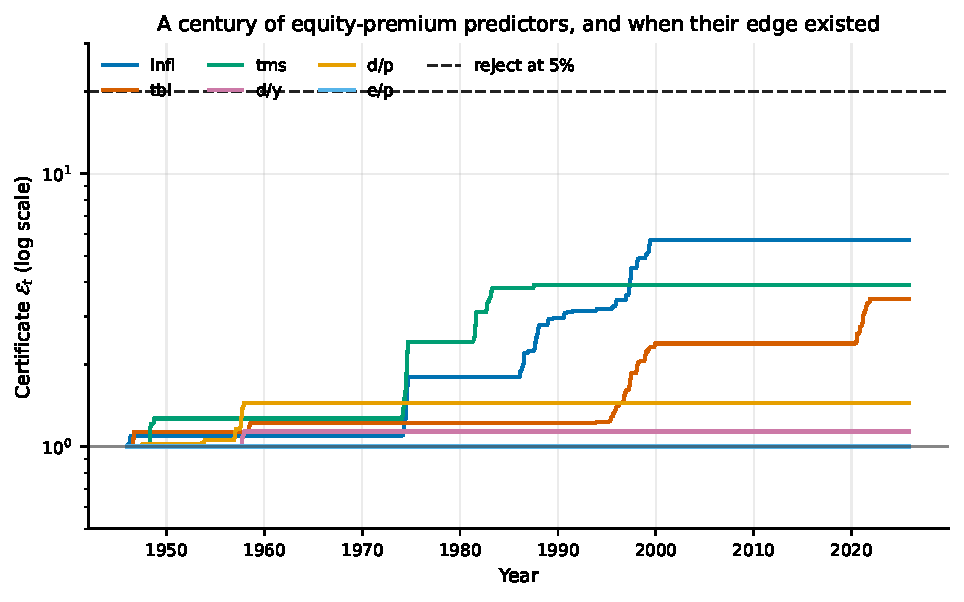
\includegraphics[width=0.92\linewidth]{fig11_goyal_welch.pdf}
  \caption{Certificate wealth for six illustrative predictors, plotted as the \emph{underlying}
  process rather than the running maximum $\mathcal{E}_t$, so that periods of no accumulation
  appear flat or falling rather than merely level. Inflation, the Treasury-bill rate and the term
  spread accumulate, at different times and none decisively; the three valuation ratios do not.
  These are paths of a noisy stochastic process, not break-date estimates: they show when this
  procedure gathered evidence, and carry no interval on any change in the underlying process.
  Note that the three valuation ratios spend most of the window \emph{below} one: $d/p$ and
  $d/y$ rise above it only transiently in the 1950s and $e/p$ never does, so no durable evidence
  accumulates for any of them---a fact the running maximum conceals by construction.
  The six are the region of the grid where the certificate and Clark--West disagree most and are
  not representative of all $117$ pairs.}
  \label{fig:dating}
\end{figure}


\paragraph{Sample accounting.} Four counts appear in this paper and they are different objects.
Table~\ref{tab:accounting} states each once.

\begin{table}[t]
  \centering
  \caption{What each count in this paper refers to.}
  \label{tab:accounting}
  \small
  \begin{tabular}{rlp{0.52\linewidth}}
    \toprule
    Count & Object & Scope \\
    \midrule
    $117$ & Primary grid & Every predictor--frequency pair that clears the minimum-observation
    rule, run once under the pre-specified design. All rejection and merging statistics use
    this. \\
    $116$ & Unflagged pairs & The primary grid less the one degenerate fit
    (Section~\ref{sec:results}). Ceiling summaries use this, since a nine-sigma forecast makes a
    ceiling uninterpretable rather than wrong. Including it moves the median by less than
    $0.01$. \\
    $56$  & Own-sample audit & Variables in \citeauthor{goyal2024}'s ReadMe with a recorded
    sample period from which a span can be computed; the audit is per \emph{variable}, not per
    pair. \\
    $14$  & Sensitivity grid & The classic monthly predictors, re-run under nine designs. \\
    \bottomrule
  \end{tabular}
\end{table}

\subsection{Does the standard toolkit see anything we do not?}
\label{sec:toolkit}

A non-result from a new instrument is worth little until the conventional instruments have been
run on identical inputs. Table~\ref{tab:toolkit} does that on the fourteen classic monthly
predictors, using the same walk-forward forecasts.

Diebold--Mariano on squared-error loss is reported for completeness and is \emph{not} a valid
test here: the comparison is nested, so under the null the loss differential is degenerate and
the statistic is not asymptotically normal \citep{clark2001}. It rejects nothing, and it would
be no evidence if it did. Clark--West, the standard nested correction, rejects nothing at $5\%$;
its largest statistic is $1.64$ for $d/y$, a one-sided $p$ of $0.051$, which is not significant
before any multiplicity correction and is far from it after. The Clark--McCracken ENC-t
statistic is, for a one-step-ahead nested pair, \emph{algebraically identical} to Clark--West:
the adjusted loss differential is exactly twice the encompassing product and the factor cancels
in the $t$-ratio. We verify this to machine precision in code and report it as one test rather
than two, because presenting the same number under two names would overstate the corroboration.

The model confidence set of \citet{hansen2011}, computed over the benchmark and all fourteen
models jointly with a stationary bootstrap, retains \emph{all fifteen} at the $90\%$ level. That
is the sharpest way to state the situation: after eighty years of monthly data, the historical
mean cannot be distinguished from any predictor in the classic set, nor any predictor from any
other. The MCS and the grid-level e-value answer the same question and give the same answer.

None of this makes the certificate right. It establishes the weaker thing the paper needs: the
absence of a rejection is a property of the data at this sample size, not of our instrument, and
the toolkit that produced the literature's positive results does not produce them here. What the
toolkit does not supply, at any point, is a bound on how large the effect could still be. That
is the gap the ceiling fills.

\begin{table}[t]
  \centering
  \caption{The conventional toolkit on the identical walk-forward forecasts, fourteen classic
  monthly predictors, $960$ monthly observations each. DM is shown for completeness only and is
  invalid under nesting. ENC-t coincides with Clark--West by construction. No test rejects at
  $5\%$ uncorrected, let alone corrected.}
  \label{tab:toolkit}
  \small
  \begin{tabular}{lrrrrr}
    \toprule
    Predictor & DM (invalid) & $p$ & Clark--West $=$ ENC-t & $p$ & In MCS \\
    \midrule
    $d/p$  & $-0.16$ & $0.56$ & $1.34$  & $0.090$ & yes \\
    $d/y$  & $-0.73$ & $0.77$ & $1.64$  & $0.051$ & yes \\
    $e/p$  & $-0.73$ & $0.77$ & $1.55$  & $0.060$ & yes \\
    $d/e$  & $-1.33$ & $0.91$ & $-0.37$ & $0.644$ & yes \\
    $b/m$  & $-1.41$ & $0.92$ & $0.59$  & $0.279$ & yes \\
    $ntis$ & $-0.40$ & $0.66$ & $0.86$  & $0.195$ & yes \\
    $tbl$  & $0.09$  & $0.47$ & $1.44$  & $0.075$ & yes \\
    $lty$  & $-0.53$ & $0.70$ & $1.37$  & $0.085$ & yes \\
    $ltr$  & $-1.80$ & $0.96$ & $-0.56$ & $0.713$ & yes \\
    $tms$  & $-0.17$ & $0.57$ & $0.78$  & $0.217$ & yes \\
    $dfy$  & $-0.93$ & $0.82$ & $-0.75$ & $0.774$ & yes \\
    $dfr$  & $-0.87$ & $0.81$ & $-0.23$ & $0.591$ & yes \\
    $infl$ & $0.39$  & $0.35$ & $0.83$  & $0.203$ & yes \\
    $svar$ & $-0.63$ & $0.74$ & $-0.51$ & $0.696$ & yes \\
    \midrule
    \multicolumn{6}{l}{Benchmark (historical mean) is also retained: $15$ of $15$ models in the
    $90\%$ MCS.} \\
    \bottomrule
  \end{tabular}
\end{table}

\subsection{Could the samples ever have supported the claims?}
\label{sec:audit}

The bound is a statement about a sample, so it can be applied retrospectively. Every variable
in the set has a recorded data span, that span fixes the floor any test faces on it, and the
comparison with a claimed effect is then arithmetic rather than opinion.

Table~\ref{tab:audit} does this for the $56$ variables with a recorded sample. Of those,
$23$---$41\%$---have a span too short to certify an annualised ratio of $0.25$ even as a single
test at the $5\%$ level. Once the $46$-variable search that generated the set is corrected for,
the figure is $56$ of $56$. The median span is $99$ years and the median corrected floor is
$0.39$, against a target of $0.25$.

\paragraph{The result does not rest on a punitive correction.} Bonferroni is the most
conservative multiplicity adjustment in common use, so it is fair to ask whether the headline
is an artifact of choosing it. It is not, for a structural reason: at the \emph{first}
rejection both Holm and Benjamini--Hochberg use the same threshold $\alpha/m$ that Bonferroni
uses everywhere, and the question is whether \emph{any} variable in the set clears the bar. All three therefore give $0$ of $56$ below $0.25$. So does a merely stricter single
test at $\alpha=0.01$ with no multiplicity adjustment at all. And with \emph{no} correction
whatsoever, $23$ of $56$ still fail. The finding depends on there being forty-six tests, not
on how one chooses to price them.

The direction of the shortfall is the unfavourable one. The shortest samples belong to the
newest variables: the risk-neutral variance measures span under thirty years and face a solo
floor of $0.46$, nearly twice the effect they would need to establish. A literature that adds
variables faster than it adds data moves away from the threshold, not towards it.

\begin{table}[t]
  \centering
  \caption{The minimum detectable ratio implied by each variable's own sample span, at $80\%$
  power, for the twelve
  shortest-sampled. ``Solo'' is a single test at $5\%$; ``corrected'' applies Bonferroni over
  the $46$-variable search. Both are compared against an annualised information ratio of
  $0.25$.}
  \label{tab:audit}
  \small
  \begin{tabular}{llrrr}
    \toprule
    Variable & Frequency & Span (years) & Floor, solo & Floor, corrected \\
    \midrule
    rsvix  & Monthly   & $29.6$ & $0.46$ & $0.72$ \\
    impvar & Monthly   & $29.6$ & $0.46$ & $0.72$ \\
    vp     & Monthly   & $31.9$ & $0.44$ & $0.69$ \\
    vrp    & Monthly   & $34.9$ & $0.42$ & $0.66$ \\
    crdstd & Quarterly & $35.5$ & $0.42$ & $0.66$ \\
    disag  & Monthly   & $44.0$ & $0.37$ & $0.59$ \\
    shtint & Monthly   & $52.9$ & $0.34$ & $0.54$ \\
    sntm   & Monthly   & $58.3$ & $0.33$ & $0.51$ \\
    accrul & Annual    & $60.0$ & $0.32$ & $0.50$ \\
    cfacc  & Annual    & $60.0$ & $0.32$ & $0.50$ \\
    csp    & Monthly   & $65.6$ & $0.31$ & $0.48$ \\
    ndrbl  & Monthly   & $67.8$ & $0.30$ & $0.47$ \\
    \midrule
    \multicolumn{5}{l}{Median over all $56$: span $99$ y, solo $0.25$, corrected $0.39$} \\
    \multicolumn{5}{l}{Below $0.25$: solo $33/56$; corrected $0/56$ under Bonferroni,} \\
    \multicolumn{5}{l}{\quad Holm and Benjamini--Hochberg alike} \\
    \bottomrule
  \end{tabular}
\end{table}

\subsection{How much of the time was each edge present?}
\label{sec:duty}

Proposition~\ref{prop:intermittent} needs a measured duty cycle to bite. We take it from the
certificate's underlying process---not from $\mathcal{E}_t$, which is a running maximum and so
rises only when a new high is set---by splitting each evaluation window into ten equal
sub-periods and recording the fraction in which log wealth increased. A predictor with no edge
scores about one half.

The median across $116$ predictors is $0.40$, with quartiles $0.30$ and $0.50$: slightly
\emph{below} the one-half baseline a no-edge process produces, which is what a set of variables
with no reliable edge looks like. We do not read a duty cycle off the year each wealth path
peaks; per Remark~\ref{rem:nophi} that quantity is post-hoc and carries no interval.

Treating $0.40$ as a hypothetical $\phi$ and feeding it through
Proposition~\ref{prop:intermittent} multiplies the required span by $2.5$, equivalently the
required ratio by $\sqrt{2.5}=1.58$. Combined with the corrected floor of $0.39$ from
Table~\ref{tab:audit}, a variable that was genuinely present only two-fifths of the time would
need an on-period annualised information ratio near $0.6$---more than twice the threshold for
economic significance---for its own sample to have established it. We offer this as an
illustration of the direction and magnitude of the intermittency penalty, not as an estimate:
the descriptive statistic above is not an estimator of $\phi$, and we make no claim that it
is.

\paragraph{One degenerate fit, flagged rather than trusted.} The variance risk premium at
quarterly frequency reports $\rsq=-98\%$ alongside an e-value of $4.76$. This is not a
contradiction: its regression forecasts a $-78\%$ quarterly equity premium against an outcome
standard deviation of $8\%$, a nine-sigma artifact of a $120$-observation fit. Squared-error
measures are quadratic and one such point destroys them; the certificate's stake is capped
relative to the signal's own scale and is unmoved. We record the largest forecast each fit
ever made in units of the outcome's standard deviation and flag anything beyond five. One of
$117$ is flagged; excluding it changes nothing.

\section{Discussion}

\paragraph{A null result and a bound are different objects.} \citet{welch2008} established
that these predictors do not beat the historical mean out of sample, and we reproduce it. What
that literature has not supplied is the other half: how large an effect the data could have
excluded. Without it a negative result is not interpretable, because it is consistent both
with there being nothing and with there being something the design could never have seen.
Table~\ref{tab:floor} shows this literature has lived in the second case throughout.

\paragraph{The instrument is not the finding.} We are explicit that the certificate is less
powerful than Clark--West where Clark--West is well specified \citep{guven2026}. It is used
here for three things a $t$-statistic cannot do: produce a time-uniform ceiling, show where in
the sample evidence accumulated, and correct a dependent grid without a bootstrap. Its failure to certify is therefore weak evidence on its
own, and the ceilings---which do not depend on rejecting anything---carry the paper.

\paragraph{What would change the answer.} Not, within the Gaussian benchmark,
a test of the same size and power: Proposition~\ref{prop:floor} fixes the detectable effect
from the span alone. Not finer sampling:
Corollary~\ref{cor:frequency}. Only a longer span, a larger effect, or a smaller search. Of
those, only the last is under a researcher's control, which is an argument for pre-registering
a small number of candidates rather than screening many.

\section{Limitations}

The floor of Proposition~\ref{prop:floor} assumes a constant effect; a predictor that is
strong in some regimes and absent in others has a higher effective floor still, so our numbers
are optimistic. Bonferroni is conservative, and a sharper multiplicity correction would lower
the corrected column of Table~\ref{tab:floor}, though not to the point of clearing the
boundary. The certificate's own conservatism means its ceilings are wider than a
fixed-sample interval would be, which cuts against us. And our predictor set is
\citeauthor{goyal2024}'s: a set assembled from published papers is selected on past
significance, which biases toward finding predictability, not away from it.

\section{Conclusion}

Evidence about an alpha accumulates as log wealth, so under a Gaussian constant-effect
benchmark what a design can detect is fixed in advance by its evaluation span, its size, its
target power and the breadth of the search. For the canonical equity-premium data those
quantities require $103$ years of evaluation for a single prespecified predictor against the
effect this literature calls economically significant, and $253$ once the search
\citet{goyal2024} actually ran is priced. The 1926--2025 data, after a twenty-year burn-in,
supply eighty.

Applying an anytime-valid certificate to $117$ predictor--frequency pairs certifies nothing,
under the primary specification or under any of nine variants. That non-result is the expected
one and is not the contribution. The contribution is the interval the certificate supplies
without needing to reject: across the $116$ unflagged pairs the median marginal $95\%$ upper
endpoint on the incremental annualised information ratio is $0.60$, and $112$ exceed $0.25$.
A century of the best-studied data in finance leaves most of these predictors compatible both
with no predictability at all and with roughly twice as much as would matter. The sequential
paths add a description of when each procedure gathered its evidence---never, for the three
valuation ratios the literature cites most; late and unevenly for inflation, the Treasury-bill
rate and the term spread---which a covariance averaged over the same century cannot show. We
report that as heterogeneity in evidence accumulation. Whether it
reflects a change in the underlying process is a question this design cannot answer, and we do
not claim it does.

\appendix

\section{Every predictor}
\label{app:full}

Table~\ref{tab:full} reports all $117$ predictor--frequency pairs. ``Source'' records whether
the predictor is the real-time diagonal of a \citet{goyal2024} vintage matrix or the workbook
column. A dagger marks the single fit flagged as degenerate---a forecast beyond five outcome
standard deviations---which is excluded from the summary statistics in the body and changes
none of them.

\begin{table}[hbtp]
  \centering
  \caption{All predictor--frequency pairs, 1926--2025. Rejecting needs an e-value of $20$;
  the largest observed is $7.47$. ``Ceiling'' is the $95\%$ anytime-valid upper bound on the
  incremental annualised information ratio.}
  \label{tab:full}
  \scriptsize
  \begin{tabular}{llrrrrr}
    \toprule
    Predictor & Source & $n$ & $\rsq$ (\%) & Clark--West & e-value & Ceiling \\
    \midrule
    \multicolumn{7}{l}{\emph{Annual}} \\
    ogap & workbook & 80 & $3.66$ & $2.54$ & $4.96$ & $1.48$ \\
    ndrbl & workbook & 57 & $7.30$ & $2.28$ & $3.14$ & $2.17$ \\
    tail & workbook & 80 & $-0.28$ & $0.29$ & $2.60$ & $0.49$ \\
    gpce & real time & 68 & $9.53$ & $2.00$ & $2.59$ & $1.47$ \\
    ltr & workbook & 80 & $-7.67$ & $1.65$ & $2.13$ & $0.53$ \\
    pce & workbook & 62 & $10.75$ & $3.22$ & $2.13$ & $1.28$ \\
    lzrt & workbook & 80 & $-2.36$ & $1.46$ & $2.07$ & $0.91$ \\
    eqis & workbook & 80 & $0.67$ & $1.59$ & $1.93$ & $1.18$ \\
    d/p & workbook & 80 & $0.22$ & $0.97$ & $1.83$ & $0.76$ \\
    lty & workbook & 80 & $-6.44$ & $0.94$ & $1.66$ & $0.99$ \\
    govik & workbook & 68 & $-3.61$ & $1.04$ & $1.64$ & $1.13$ \\
    i/k & workbook & 68 & $4.89$ & $2.05$ & $1.58$ & $1.25$ \\
    tbl & workbook & 80 & $-4.59$ & $0.79$ & $1.55$ & $1.09$ \\
    skvw & workbook & 80 & $-0.12$ & $0.51$ & $1.54$ & $0.79$ \\
    fbm & workbook & 80 & $-1.26$ & $-1.04$ & $1.46$ & $0.76$ \\
    d/y & workbook & 80 & $-0.22$ & $1.35$ & $1.37$ & $0.55$ \\
    d/e & workbook & 80 & $-2.91$ & $-0.69$ & $1.37$ & $0.62$ \\
    accrul & real time & 50 & $6.68$ & $1.36$ & $1.32$ & $2.12$ \\
    b/m & workbook & 80 & $-8.12$ & $0.87$ & $1.27$ & $0.80$ \\
    dfr & workbook & 80 & $-3.95$ & $-0.18$ & $1.26$ & $0.68$ \\
    e/p & workbook & 80 & $0.95$ & $1.82$ & $1.26$ & $0.59$ \\
    tchi & workbook & 64 & $-4.83$ & $-0.68$ & $1.25$ & $0.63$ \\
    svar & workbook & 80 & $-0.18$ & $-0.23$ & $1.16$ & $0.78$ \\
    sntm & workbook & 48 & $-15.16$ & $0.06$ & $1.15$ & $1.06$ \\
    wtexas & workbook & 80 & $-4.34$ & $0.81$ & $1.15$ & $1.22$ \\
    gip & real time & 80 & $-1.86$ & $-1.11$ & $1.13$ & $0.11$ \\
    disag & workbook & 34 & $-11.30$ & $0.08$ & $1.11$ & $3.67$ \\
    skew & workbook & 59 & $-2.91$ & $-0.14$ & $1.10$ & $1.13$ \\
    cfacc & real time & 50 & $7.69$ & $3.34$ & $1.09$ & $2.66$ \\
    ntis & workbook & 80 & $-6.87$ & $0.27$ & $1.09$ & $1.06$ \\
    dtoat & workbook & 80 & $-1.33$ & $-0.34$ & $1.05$ & $0.64$ \\
    cay & workbook & 70 & $-2.99$ & $0.22$ & $1.03$ & $1.34$ \\
    house & real time & 80 & $-1.04$ & $0.26$ & $1.01$ & $0.38$ \\
    rdsp & workbook & 80 & $-0.93$ & $0.33$ & $1.01$ & $0.71$ \\
    dfy & workbook & 80 & $-0.90$ & $-0.76$ & $1.01$ & $0.61$ \\
    avgcor & workbook & 80 & $-7.10$ & $-0.71$ & $1.01$ & $0.46$ \\
    dtoy & workbook & 80 & $-6.60$ & $-0.79$ & $1.01$ & $0.43$ \\
    ygap & workbook & 62 & $-11.46$ & $0.30$ & $1.00$ & $1.07$ \\
    shtint & workbook & 42 & $-24.60$ & $-1.58$ & $1.00$ & $2.04$ \\
    csp & workbook & 56 & $-8.65$ & $-0.97$ & $1.00$ & $0.60$ \\
    infl & workbook & 80 & $-5.93$ & $-1.53$ & $1.00$ & $0.30$ \\
    tms & workbook & 80 & $-3.15$ & $0.40$ & $1.00$ & $1.07$ \\
    \midrule
    \multicolumn{7}{l}{\emph{Monthly}} \\
    wtexas & real time & 960 & $0.01$ & $1.85$ & $7.47$ & $0.35$ \\
    sntm & workbook & 641 & $0.42$ & $2.03$ & $5.92$ & $0.66$ \\
    ogap & real time & 960 & $0.26$ & $1.73$ & $5.77$ & $0.46$ \\
    infl & workbook & 960 & $0.11$ & $0.83$ & $5.71$ & $0.51$ \\
    ndrbl & real time & 743 & $-0.09$ & $0.99$ & $4.57$ & $0.62$ \\
    csp & workbook & 685 & $-1.05$ & $2.07$ & $4.30$ & $0.46$ \\
    tms & workbook & 960 & $-0.08$ & $0.78$ & $3.92$ & $0.78$ \\
    tbl & workbook & 960 & $0.07$ & $1.44$ & $3.48$ & $0.91$ \\
    ntis & workbook & 960 & $-0.33$ & $0.86$ & $2.84$ & $0.60$ \\
    disag & real time & 468 & $-0.66$ & $-0.31$ & $2.11$ & $0.99$ \\
    vrp & real time & 360 & $-6.20$ & $-0.04$ & $2.04$ & $1.31$ \\
    lzrt & real time & 960 & $-0.17$ & $0.66$ & $1.93$ & $0.40$ \\
    lty & workbook & 960 & $-0.60$ & $1.38$ & $1.91$ & $0.54$ \\
    dtoat & real time & 960 & $-0.07$ & $-0.20$ & $1.70$ & $0.62$ \\
    d/e & workbook & 960 & $-1.52$ & $-0.37$ & $1.47$ & $0.42$ \\
    d/p & workbook & 960 & $-0.10$ & $1.34$ & $1.45$ & $0.46$ \\
    dfy & workbook & 960 & $-0.11$ & $-0.75$ & $1.40$ & $0.38$ \\
    fbm & workbook & 960 & $-1.57$ & $0.17$ & $1.33$ & $0.42$ \\
    rdsp & real time & 960 & $-0.06$ & $-0.53$ & $1.26$ & $0.44$ \\
    tchi & real time & 779 & $-0.07$ & $0.51$ & $1.24$ & $0.70$ \\
    svar & workbook & 960 & $-0.30$ & $-0.51$ & $1.24$ & $0.41$ \\
    dtoy & real time & 960 & $-0.55$ & $-0.53$ & $1.23$ & $0.43$ \\
    rsvix & workbook & 296 & $-3.11$ & $-0.81$ & $1.16$ & $0.89$ \\
    impvar & real time & 296 & $-1.79$ & $0.14$ & $1.15$ & $1.12$ \\
    d/y & workbook & 960 & $-0.75$ & $1.64$ & $1.14$ & $0.41$ \\
    tail & real time & 960 & $-0.37$ & $-0.52$ & $1.08$ & $0.36$ \\
    skvw & real time & 960 & $-0.61$ & $-1.32$ & $1.04$ & $0.18$ \\
    avgcor & real time & 960 & $-0.17$ & $-0.18$ & $1.02$ & $0.38$ \\
    vp & real time & 324 & $0.07$ & $0.63$ & $1.02$ & $1.10$ \\
    ltr & workbook & 960 & $-0.99$ & $-0.56$ & $1.00$ & $0.27$ \\
    e/p & workbook & 960 & $-0.79$ & $1.55$ & $1.00$ & $0.40$ \\
    b/m & workbook & 960 & $-1.35$ & $0.59$ & $1.00$ & $0.46$ \\
    shtint & real time & 515 & $-0.15$ & $0.99$ & $1.00$ & $1.00$ \\
    ygap & real time & 812 & $-1.02$ & $-0.46$ & $1.00$ & $0.39$ \\
    dfr & workbook & 960 & $-0.43$ & $-0.23$ & $1.00$ & $0.36$ \\
    \midrule
    \multicolumn{7}{l}{\emph{Quarterly}} \\
    i/k & workbook & 295 & $2.94$ & $3.19$ & $5.87$ & $0.65$ \\
    sntm & workbook & 213 & $1.42$ & $2.28$ & $5.33$ & $0.64$ \\
    ogap & workbook & 320 & $1.10$ & $3.32$ & $4.84$ & $0.93$ \\
    vrp$^\dagger$ & workbook & 120 & $-98.38$ & $-0.28$ & $4.76$ & $1.74$ \\
    cay & workbook & 275 & $-3.15$ & $0.87$ & $2.96$ & $0.45$ \\
    crdstd & real time & 122 & $-0.18$ & $1.08$ & $2.68$ & $1.66$ \\
    lzrt & workbook & 320 & $-3.02$ & $0.59$ & $1.78$ & $0.36$ \\
    tms & workbook & 320 & $-0.47$ & $0.41$ & $1.78$ & $0.79$ \\
    csp & workbook & 229 & $-0.72$ & $0.01$ & $1.77$ & $0.50$ \\
    tbl & workbook & 320 & $-0.15$ & $1.13$ & $1.61$ & $0.88$ \\
    vp & workbook & 108 & $4.67$ & $1.80$ & $1.59$ & $1.66$ \\
    wtexas & workbook & 320 & $-2.80$ & $0.22$ & $1.46$ & $0.37$ \\
    avgcor & workbook & 320 & $0.92$ & $1.59$ & $1.44$ & $0.53$ \\
    lty & workbook & 320 & $-1.86$ & $1.01$ & $1.44$ & $0.60$ \\
    rsvix & workbook & 98 & $-5.70$ & $0.54$ & $1.38$ & $0.95$ \\
    ntis & workbook & 320 & $-2.32$ & $0.67$ & $1.36$ & $0.63$ \\
    dtoat & workbook & 320 & $-0.10$ & $0.18$ & $1.36$ & $0.61$ \\
    govik & real time & 295 & $-0.74$ & $1.09$ & $1.34$ & $0.50$ \\
    ndrbl & workbook & 248 & $-0.49$ & $0.82$ & $1.25$ & $0.56$ \\
    disag & workbook & 156 & $-1.71$ & $0.21$ & $1.22$ & $1.52$ \\
    d/p & workbook & 320 & $-1.29$ & $1.61$ & $1.22$ & $0.42$ \\
    dfy & workbook & 320 & $-0.45$ & $-0.25$ & $1.20$ & $0.52$ \\
    d/e & workbook & 320 & $-4.88$ & $-0.60$ & $1.17$ & $0.38$ \\
    impvar & workbook & 98 & $-3.54$ & $0.37$ & $1.17$ & $1.84$ \\
    dtoy & workbook & 320 & $-1.18$ & $-1.01$ & $1.13$ & $0.40$ \\
    d/y & workbook & 320 & $-3.06$ & $1.73$ & $1.12$ & $0.40$ \\
    fbm & workbook & 320 & $-4.10$ & $0.01$ & $1.09$ & $0.46$ \\
    pce & real time & 256 & $-1.45$ & $0.09$ & $1.06$ & $0.36$ \\
    dfr & workbook & 320 & $-5.60$ & $-2.14$ & $1.05$ & $0.15$ \\
    rdsp & workbook & 320 & $-0.24$ & $0.44$ & $1.01$ & $0.56$ \\
    ygap & workbook & 270 & $-2.96$ & $-0.16$ & $1.00$ & $0.50$ \\
    shtint & workbook & 191 & $-3.73$ & $-1.87$ & $1.00$ & $0.45$ \\
    ltr & workbook & 320 & $0.52$ & $1.24$ & $1.00$ & $0.69$ \\
    infl & workbook & 320 & $-0.32$ & $-0.65$ & $1.00$ & $0.41$ \\
    svar & workbook & 320 & $-0.26$ & $-1.46$ & $1.00$ & $0.56$ \\
    tail & workbook & 320 & $-0.68$ & $-0.79$ & $1.00$ & $0.26$ \\
    b/m & workbook & 320 & $-5.72$ & $0.87$ & $1.00$ & $0.53$ \\
    skvw & workbook & 320 & $-4.96$ & $-2.03$ & $1.00$ & $0.21$ \\
    e/p & workbook & 320 & $-4.22$ & $1.68$ & $1.00$ & $0.38$ \\
    tchi & workbook & 279 & $-1.28$ & $-0.31$ & $1.00$ & $0.41$ \\
    \bottomrule
\end{tabular}

\end{table}

\bibliographystyle{unsrtnat}
\bibliography{references}

\end{document}
